\section{Relations Between the Models}
\label{sec:comp}

In order to create the $\mathcal{F}_1$ model, it is necessary to express variables  $X^s_{ij}$ in $\mathcal{F}_1$ space using relation (\ref{eq:tr:xijj}).
The aim of this section is to show how the entire $\mathcal{X}_2$ model can be converted into an equivalent model that uses only variables of $\mathcal{F}_2$.
 

The following equations express all variables from $\mathcal{X}_2$ in $\mathcal{F}_2$ space:
%%%%%%%%%%%%%%%%%%%%%%%%%%%%%%%%%%%%%%%
%                                     % 
%       Transformation (7)            %
%                                     %
%%%%%%%%%%%%%%%%%%%%%%%%%%%%%%%%%%%%%%%
\begin{subequations}
\begin{align}
\notag\label{eq:tr:fstij}x^{st}_{ij}&=F^t_{ij}(1- f^{st}_{ij})+F^s_{ji}(1- f^{st}_{ji})= \\
  &=  F^t_{ij}+F^s_{ji} -  f^{st}_{ij} -  f^{st}_{ji}& (i,j)\in A, \{s,t\}\in S_0\\
\notag\label{eq:tr:xijj}X^s_{ij}&=g_{ij}(1-F^s_{ij})(1-F^s_{ji})+g_{ji}F^s_{ji}=\\
  &= g_{ij}-F^s_{ij} + F^s_{ji} & (i,j)\in A, s\in D_0\\
\label{eq:tr:zij}y_{ij}&=g_{ij}+g_{ji}& \{i,j\}\in E
\end{align}
\end{subequations}
The transformations can be explained as follows:
Let $T=(V_T,E_T)$ be a tree covering $D$, and consider an edge $\{i,j\}\in E_T$ dividing $T$ into two subtrees $T_i$ and $T_j$ rooted in $i$ and $j$, respectively.
If the arc $(i,j)$ carries flow from $s\in D$ to $t\in D$, then $s$ and $t$ must lie in different subtrees.
Node $s_0$ lies either in $T_i$ or $T_j$.
%as depicted in Fig. \ref{fig:transf_a} and Fig. \ref{fig:transf_b}, respectively.
These two cases are captured by the first equality in (\ref{eq:tr:fstij}).
If both $s_0$ and $s$ lie in $T_i$, then $F^t_{ij}=1$.
Similarly, if $s_0$ and $t$ lie in $T_j$, then $F_{ji}^s=1$.
The expressions in parentheses prevent $s$ and $t$ belonging to the same subtree.
Using the implications $f^{st}_{ij}=1\Rightarrow F^t_{ij}=1$ and $f^{st}_{ji}=1\Rightarrow F_{ji}^s=1$ that follow from the interpretation of variables, we justify the second equality expressing this relation linearly.
In the transformation (\ref{eq:tr:xijj}) of $g_{ij}^s$, we distinguish the situation when $s_0$ and $s$ are in the same subtree, in which case none of the arcs $(i,j)$ and $(j,i)$ carries a flow to $s$, and when $s$ and $s_0$ belong to different subtrees, and there is a flow via $(j,i)$ towards $s$.
Again, the last equality is justified since $F_{ij}^s=1\Rightarrow g_{ij}=1$.
The relation (\ref{eq:tr:zij}) is obvious.

By a similar approach, we achieve the transformation from $\mathcal{X}_2$ space to $\mathcal{F}_2$ space. 
%%%%%%%%%%%%%%%%%%%%%%%%%%%%%%%%%%%%%%%
%                                     %
%       Transformation (8)            %
%                                     %
%%%%%%%%%%%%%%%%%%%%%%%%%%%%%%%%%%%%%%%
\begin{subequations}
\begin{align}
\label{eq:tr:xij=xij0}g_{ij}=&x^0_{ij} & (i,j)\in A\\
\label{eq:tr:fijt2}F^t_{ij}=&x^t_{ji}x^0_{ij}=f^{0t}_{ij} & (i,j)\in A, t\in D_0\\
\label{eq:tr:fstij2} f^{st}_{ij}=& x^s_{ji}x^t_{ji}x^0_{ij} & (i,j)\in A, \{s,t\}\in \check{S}_0
\end{align}
\end{subequations}

We aim to compare the models presented in Section \ref{sec:ILP} in terms of strength.
The results obtained by numerical experiments presented in the next section suggest that $\mathcal{F}_2$ model is at least as strong as $\mathcal{X}_2$.
This section proves this conjecture.
 
First, we express the $\mathcal{X}_2$ model in $\mathcal{F}_2$ space using transformations (\ref{eq:tr:fstij})-(\ref{eq:tr:zij}). 
%%%%%%%%%%%%%%%%%%%%%%%%%%%%%%%%%%%%%%%
%                                     %
%             MODEL (9)               %
%                                     %
%%%%%%%%%%%%%%%%%%%%%%%%%%%%%%%%%%%%%%%
\begin{subequations}
\begin{flalign}
\label{objective:mfinpf2} &\makebox[0pt][l]{$\displaystyle{}\min \sum\limits_{(i,j) \in A} \sum\limits_{s \in D} p_{ij} \pi^s_{ij} $} & \\ 
\notag\text{s.t.}& & \\
\label{con:mfinpf2:arrowFromDest} \sum\limits_{j\in V_i}(g_{ji}-F^s_{ji}+F^s_{ij}) & = 1 & i\in D, s\in D, i \neq s,\\ 
\label{con:mfinpf2:arrowFromNonDestB} \sum\limits_{j \in V_i}(g_{ji}-F^s_{ji}+F^s_{ij}) &\leq 1 & i\in V \setminus D, s\in D,\\
\label{con:mfinpf2:arrowFromNonDestA} g_{ij}-F^s_{ij}+F^s_{ji}  & \leq \sum\limits_{k \in V_i\setminus\{j\}}(g_{ki}-F^s_{ki}+F^s_{ik}) & i\in V \setminus D,\\
\notag & & j\in V_i, s\in D,\\
\label{con:mfinpf2:startInSource} x_{js} - F^s_{js}+F^s_{sj} & = 0 & s\in D, j\in V_s,\\
\label{con:mfinpf2:yvar} g_{ij}-F^s_{ij}+F^s_{ji} & \leq \sum\limits_{k\in V:p_{ik}\geq p_{ij}}\pi^s_{ik} & s\in D, (i,j)\in A,\\ 
\label{con:mfinpf2:extraCon} \sum\limits_{j\in V_{i}}\left(g_{ji}-F^s_{ji}+F^s_{ij}\right) & \leq \sum\limits_{j\in V_{i}}\left(g_{ij}-F^s_{ji}+F^s_{ij}\right)  &\in V\setminus D, s\in D,\\
\notag\text(\ref{con:vi:Y1}) & &\\
\label{con:mfinpf2:sumYImpSumXTrans} \sum\limits_{j\in V_i\setminus\{s\} }\pi^{s}_{ij} & \geq \sum\limits_{j\in V_i} \left( g_{ji}-F^s_{ji}+F^s_{ij} \right) &  i\in V\setminus D, s\in D,\\ 
\label{con:mfinpf2:flowNormal}  \sum\limits_{\substack{ j\in V_i }}(F^t_{ij}+F^s_{ji})&=\sum\limits_{\substack{j\in V_i }}(F^t_{ji}+F^s_{ij}) & i\in V, t\in D, i \neq t,\\
\label{con:mfinpf2:flowDest}  \sum\limits_{\substack{j\in V_t}}(F^t_{tj}+F^s_{jt})&=\sum\limits_{\substack{j\in V_t}}(F^t_{jt}+F^s_{tj})  = -1  &  t \in D,\\
\label{con:mfinpf2:zbound} g_{ij}+g_{ji}&\leq 1 & \{i,j\}\in E, \\
\label{con:mfinpf2:xbound} 0&\leq g_{ij}-F_{ij}^s+F_{ji}^s  \leq 1 & (i,j)\in A, s\in D,\\
\label{con:mfinpf2:fcap} F^t_{ij} -  f^{st}_{ij} -  f^{st}_{ji} &\leq  g_{ij}-F^s_{ij} & (i,j)\in A, \{s,t\}\in \check{S},\\
\label{con:mfinpf2:fbound} 0  \leq F^t_{ij}+F_{ji}^s & - f_{ij}^{st}- f_{ji}^{st}  \leq 1 & \{i,j\}\in E,\{s,t\}\in \check{S},\\
\label{con:mfinpf2:fij00} F^0_{ij} &=0 & (i,j)\in A,\\
\label{con:mfinpf2:dim} g \in \{0,1\}^{A},F&\in\{0,1\}^{A \times D}, f\in\{0,1\}^{A\times \check{S}},\\
\label{con:mfinpf2:dimy} \pi &\in \{0,1\}^{A\times D}.
\end{flalign}
\end{subequations}

%Note that the 4-index variables $ f^{st}_{ij}$ appear only in (\ref{con:mfinpf2:fcap}) and (\ref{con:mfinpf2:fbound}). Assigning the highest possible values $ f^{st}_{ij}=F^{t}_{ij}$ and $ f^{st}_{ji}=F^s_{ji}$ according to (\ref{con:mfinpf2:fbound}) does not cause a violation of any other constraint. In this case (\ref{con:mfinpf2:fcap}) becomes the same as the first inequality in (\ref{con:mfinpf2:xbound}). It is therefore possible to remove (\ref{con:mfinpf2:fcap}) and (\ref{con:mfinpf2:fbound}), resulting in a model in $\mathcal{F}_1$ space (with up to 3-index variables).% equivalent to the $\mathcal{X}_2$ model. 
The following lemmata are useful for analysis of the relations between the models. 
%%%%%%%%%%%%%%%%%%%%%%%%%%%%%%%%%%%%%%%
%                                     %
%         Lemma 1                     %
%                                     %
%%%%%%%%%%%%%%%%%%%%%%%%%%%%%%%%%%%%%%%
\begin{lemma}\label{lem:sumxji1}
All feasible solutions to LP($\mathcal{F}_2$) satisfy
\begin{equation}
\sum_{j\in V_i}g_{ji}=1,\quad i\in D_0.  \label{eq:sumToD} 
\end{equation}
\end{lemma}
\begin{proof}
 Utilizing first (\ref{con:pf1:fitt=xit}), next (\ref{con:pf1:flow}) for $t=i$, and finally (\ref{con:pf1:noflowFromT}), we get
$$\sum_{j\in V_i}g_{ji}=\sum_{j\in V_i}F_{ji}^i = 1+\sum_{j\in V_i}F_{ij}^i=1.$$\qed
\end{proof}
%%%%%%%%%%%%%%%%%%%%%%%%%%%%%%%%%%%%%%%
%                                     %
%         Lemma 2                     %
%                                     %
%%%%%%%%%%%%%%%%%%%%%%%%%%%%%%%%%%%%%%%
\begin{lemma}\label{lem:onedir} LP($\mathcal{F}_2$) has an optimal solution such that \newline
$\forall (i,j)\in A, t\in D_0: \min\{F^t_{ij},F^t_{ji}\} = 0.$
\end{lemma}
\begin{proof}
Assume that $\exists t\in D_0, (i,j)\in A: \min\{F^t_{ij},F^t_{ji}\} = \epsilon> 0$ in an optimal solution.
This assumption applies only for $j\neq t$ because (\ref{con:pf1:noflowFromT}) defines $F^t_{ti}=0$.
It is then possible to reduce the flow towards $t$ along the cycle $(i,j,i)$ by $\epsilon$.
Flow conservation remains satisfied because for both $i$ and $j$, entering and leaving flow towards $t$ is reduced by the same amount.
All remaining constraints are satisfied and the left-hand side of (\ref{con:pf1:yvar}) does not change because 
$$
g_{ij}-(F^t_{ij}-\epsilon)+(F^t_{ji}-\epsilon) = g_{ij}-F^t_{ij}+F^t_{ji},
$$
and thereby the objective value is not altered. Such a solution is an alternative optimal solution satisfying the property stated by this lemma.  \qed
\end{proof}
In the following, let $F^*_{ij}=\max_{t\in D_0}\{F^t_{ij}\}$.
%%%%%%%%%%%%%%%%%%%%%%%%%%%%%%%%%%%%%%%
%                                     %
%         Lemma 3                     %
%                                     %
%%%%%%%%%%%%%%%%%%%%%%%%%%%%%%%%%%%%%%%
\begin{lemma}\label{lem:oneslack} LP($\mathcal{F}_2$) has an optimal solution such that \newline
%$\forall i,j\in V: g_{ij} = F^*_{ij} \vee g_{ji}=F^*_{ji}$.
$\forall (i,j)\in A: \min\{g_{ij} - F^*_{ij}, g_{ji}-F^*_{ji}\}=0$.
\end{lemma}
\begin{proof}
If $\exists (i,j)\in A: \min\{g_{ij} - F^*_{ij}, g_{ji}-F^*_{ji}\}=\epsilon>0$, it is possible to decrease both $g_{ij}$ and $g_{ji}$ by $\epsilon$ which does not increase the objective value, and does not violate any constraint.
In particular, the left-hand side in (\ref{con:pf1:flowX}) remains unchanged after this operation.
\qed
\end{proof}
%%%%%%%%%%%%%%%%%%%%%%%%%%%%%%%%%%%%%%%
%                                     %
%         Lemma 4                     %
%                                     %
%%%%%%%%%%%%%%%%%%%%%%%%%%%%%%%%%%%%%%%
\begin{lemma}\label{lem:xequals} LP($\mathcal{F}_2$) has an optimal solution where for each arc $(i,j)\in A$, at least one of the following properties holds:
\begin{itemize}
\item\label{lem:item:noslack} $g_{ij}=F^*_{ij},$\hfill(L.\ref{lem:xequals}a)
\item\label{lem:item:slack} (\ref{con:pf1:flowX}) is satisfied with equality at $i$, i.e., $\sum_{k\in V_{i}}g_{ki}=\sum_{k\in V_i}g_{ik}$\hfill(L.\ref{lem:xequals}b)
\end{itemize}
\end{lemma}
\begin{proof}
If $F^*_{ij}=F^t_{ij}$ and $j=t$, the option (L.4a) already holds as stated by (\ref{con:pf1:fitt=xit}).
Let $j\neq t$.
By decreasing $g_{ij}$, the objective value can not increase because $g_{ij}$ appears only in the left-hand side of (\ref{con:pf1:yvar}) and (\ref{con:pf1:yvar0}) with a positive sign.
This variable can be reduced as long as it preserves feasibility of the solution.
The only constraints that could be affected by reducing $g_{ij}$ are (\ref{con:pf1:xfrel}) and (\ref{con:pf1:flowX}), and so assigning 
%
$$g_{ij}\coloneqq\max\bigg\{ F^*_{ij},\sum_{k\in V_i}g_{ki}-\sum_{k\in V_i\setminus\{j\}}g_{ik}\bigg\}$$
%
either does not change the value $g_{ij}$, or yields an alternative optimum of LP($\mathcal{F}_2$). \qed
\end{proof}
The only constraint that could prevent $g_{ij}=F^*_{ij}$ is (\ref{con:pf1:flowX}).
If flows destined for two different destinations enter $i\in V\setminus D$ along two different entering arcs, and then continue via some shared arc $(i,j)$, then $g_{ij}>F^*_{ij}$ can occur.
An example of such situation is demonstrated in Fig. \ref{fig:counterex}.

%%%%%%%%%%%%%%%%%%%%%%%%%%%%%%%%%%%%%%
%  Figure 3                          %
%  example when g_{ij} > F^*_{ij}    %
%%%%%%%%%%%%%%%%%%%%%%%%%%%%%%%%%%%%%%
\begin{figure}[h!]
        \centering
        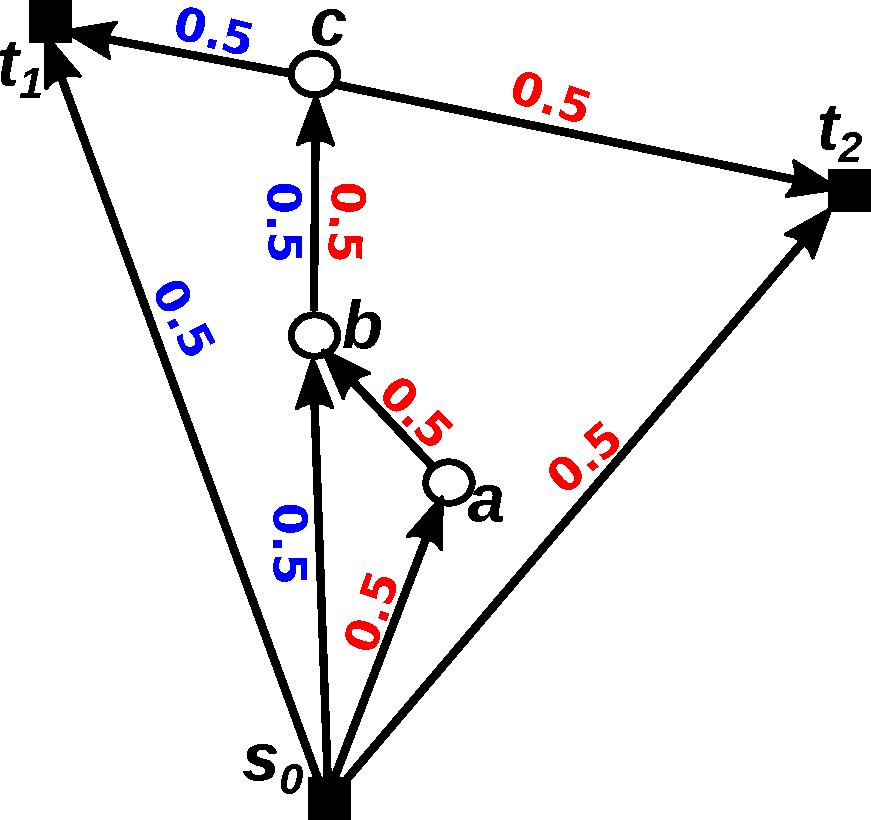
\includegraphics[height=2.3in]{counterex}
        \caption{A feasible solution to LP($\mathcal{F}_2$) of an instance on six vertices with destinations $D=\{s_0,t_1,t_2\}$.
		 Blue and red labels along the edges represent the amount of flow through a given edge towards $t_1$ and $t_2$, respectively.
		 In this solution, $g_{ij}>F^*_{ij}$, because if $x_{s_0i}=g_{ki}=0.
		5$, then $g_{ij}$ must be equal to 1 in order to fulfill (\ref{con:pf1:flowX}).}
        \label{fig:counterex}
\end{figure}
 
Consider an instance with optimal solution $(f,x,y)$ to LP($\mathcal{F}_2$) satisfying conditions in Lemma \ref{lem:onedir}.
If $(f,x,y)$ violates conditions in Lemma \ref{lem:oneslack}, it is possible to alter $x$ and obtain another optimum $(f,x',y)$ satisfying conditions in both lemmata \ref{lem:onedir} and \ref{lem:oneslack}.
Similarly, if $(f,x',y)$ still violates Lemma \ref{lem:xequals} at some arc $(i,j)$, the solution is altered by decreasing $x'_{ij}$ while preserving feasibility.
Once conditions in Lemma \ref{lem:onedir} and Lemma \ref{lem:oneslack} are satisfied, such a decrease cannot violate them.
These remarks are summarized as 
%%%%%%%%%%%%%%%%%%%%%%%%%%%%%%%%%%%%%%%
%                                     %
%         Observation 1               %
%                                     %
%%%%%%%%%%%%%%%%%%%%%%%%%%%%%%%%%%%%%%%
\begin{obs}
Instances of LP($\mathcal{F}_2$) have optimal solutions satisfying the conditions in all of Lemma \ref{lem:onedir}, Lemma \ref{lem:oneslack} and Lemma \ref{lem:xequals}.
\end{obs}
%%%%%%%%%%%%%%%%%%%%%%%%%%%%%%%%%%%%%%%
%                                     %
%         Proposition 2               %
%                                     %
%%%%%%%%%%%%%%%%%%%%%%%%%%%%%%%%%%%%%%%
\begin{prop}
\label{prop:f1strx2}
LP($\mathcal{F}_2$) is at least as strong as LP($\mathcal{X}_2$). 
\end{prop}
%%%%%%%%%%%%%%%%%%%%%%%%%%%%%%%%%%%%%%
%   Beginning of proof of Prop. 2    %
%%%%%%%%%%%%%%%%%%%%%%%%%%%%%%%%%%%%%%
\begin{proof}
Let (x,f,y) be an optimal solution to LP($\mathcal{F}_2$) satisfying the conditions in Lemmata \ref{lem:onedir}, \ref{lem:onedir} and \ref{lem:xequals}.
We show that each inequality in LP($\mathcal{X}_2$) is implied by inequalities in LP($\mathcal{F}_2$).

\begin{itemize}[leftmargin=1cm]
%\item[] (\ref{con:mfinpf2:maxsize}): Folaws directly from (\ref{eq:sumToD}) and (\ref{con:pf1:B}).
\item[ (\ref{con:mfinpf2:arrowFromDest}):] Assume $t\in D_0$ and $i\in D_0\setminus\{t\}$. Flow conservation (\ref{con:pf1:flow}) implies
	$$\sum_{j\in V_i}g_{ji} - \sum_{j\in V_i}F^t_{ji} + \sum_{j\in V_i}F^t_{ij} = \sum_{j\in V_i}g_{ji}.$$ Then (\ref{con:mfinpf2:arrowFromDest}) follows from Lemma \ref{lem:sumxji1}.
	Assume $i=s_0$. Due to (\ref{con:pf1:xi0=0}) and (\ref{con:pf1:xfrel}), the following first two sums equal zero, which gives
	$$\sum_{j\in V_i}g_{ji} - \sum_{j\in V_i}F^t_{ji} + \sum_{j\in V_i}F^t_{ij} = \sum_{j\in V_i}F^t_{ij} = 1,$$
	where the latter equality follows by summing (\ref{con:pf1:flow}) over all $i\in V\setminus\{s_0\}$. If $t=s_0$, then after applying definition (\ref{con:mfinpf2:fij00}), i. e., $F^0_{ij}=0$, (\ref{con:mfinpf2:arrowFromDest})  also follows from Lemma \ref{lem:sumxji1}. 
\item[ (\ref{con:mfinpf2:arrowFromNonDestB}):] The proof is analogous to (\ref{con:mfinpf2:arrowFromDest}), with (\ref{con:pf1:B}) replacing (\ref{eq:sumToD}).
\item[ (\ref{con:mfinpf2:arrowFromNonDestA}):] The inequality can be rewritten as
	\begin{align*}
	 g_{ij}  \leq& \sum\limits_{k \in V_i\setminus\{j\}}g_{ki}-\sum\limits_{k \in V_i\setminus\{j\}}F^s_{ki}+\sum\limits_{k \in V_i\setminus\{j\}}F^s_{ik} +F^s_{ij}-F^s_{ji} = \\
	 ~=& \sum\limits_{k \in V_i\setminus\{j\}}g_{ki}-\sum\limits_{k \in V_i}F^s_{ki}+\sum\limits_{k \in V_i}F^s_{ik} = \sum\limits_{k \in V_i\setminus\{j\}}g_{ki},
	\end{align*}
	where the last equality follows from the flow conservation (\ref{con:pf1:flow}). Now assume the contrary that for some $(i,j)\in A$, where $i\in V\setminus D$,
	\begin{align}
	g_{ij} > \sum\limits_{k \in V_i\setminus\{j\}}g_{ki}.\label{eq:assumContr}
	\end{align}
	The proof is divided into two parts that capture the two cases stated by Lemma \ref{lem:xequals}.
	Assume first that (L.4a) holds.
	We have that $\exists t\in D_0 \text{ s. t. }F^t_{ij}=g_{ij}$.
	Besides the strict inequality, assumption (\ref{eq:assumContr}) also implies $g_{ij}> 0$ which together with Lemma \ref{lem:onedir} gives $F^t_{ji}=0$.
 	By applying (\ref{con:pf1:xfrel}) to arcs entering $i$,
	$$\sum\limits_{k\in V_i}F^t_{ik} \geq F^t_{ij}=g_{ij}>\sum\limits_{k \in V_i\setminus\{j\}}g_{ki} \geq \sum\limits_{k \in V_i\setminus\{j\}}F^t_{ki}=\sum\limits_{k \in V_i}F^t_{ki},$$
	contradicting flow conservation constraints (\ref{con:pf1:flow}).
	Assume next that (L.4a) does not hold, i.e., $F^*_{ij}<g_{ij}$. 
	We know from Lemma \ref{lem:oneslack} that $g_{ji}=F^*_{ji}$, and so $\exists t\in D_0 \text{ s. t. }F^t_{ji}=g_{ji}$. 
	Moreover, Lemma \ref{lem:onedir} says that if for some $s\in D_0: F^s_{ji}>0$, then $F^s_{ij} = 0$, i.e. any flow that enters $i$ via $(j,i)$ must leave it through an arc different from $(i,j)$.
	Together with the flow conservation and (\ref{con:pf1:xfrel}),
	$$
	g_{ji}=F^t_{ji}\leq\sum_{k\in V_i}F^t_{ik}=\sum_{k\in V_i\setminus\{j\}}F^t_{ik}\leq\sum_{k\in V_i\setminus\{j\}}g_{ik}.
	$$
	Note that for $g_{ji}=F^t_{ji}=0$, $F^t_{ij}\geq 0$ in which case the second equality above would not hold, but we could directly write $g_{ji}\leq\sum_{k\in V_i\setminus\{j\}}g_{ik}$. 
	Combined with the assumption (\ref{eq:assumContr}) we obtain
	$$
	\sum_{k\in V_i}g_{ki} = g_{ji} + \sum_{k\in V_i\setminus\{j\}}g_{ki}<g_{ij} + \sum_{k\in V_i\setminus\{j\}}g_{ik} = \sum_{k\in V_i}g_{ik},
	$$
	contradicting (L.4b), and thereby Lemma \ref{lem:xequals}. 
	The proof applies with minor simplifications also for $s=s_0$.
\item[ (\ref{con:mfinpf2:startInSource}):] Follows from (\ref{con:pf1:noflowFromT}) and (\ref{con:pf1:fitt=xit}) if $s\in D_0$, or (\ref{con:pf1:xi0=0}) and (\ref{con:mfinpf2:fij00}) if $s=s_0$.
\item[ (\ref{con:mfinpf2:yvar}):] Identical to (\ref{con:pf1:yvar}) if $s\in D_0$, or follows from (\ref{con:pf1:yvar0}) and (\ref{con:mfinpf2:fij00}) if $s=s_0$.
\item[ (\ref{con:mfinpf2:extraCon}):] Follows immediately from (\ref{con:pf1:flowX}) by utilizing (\ref{con:pf1:flow}) at node $i$ if $s\in D_0$, or by utilizing (\ref{con:mfinpf2:fij00}) if $s=s_0$.
\item[(\ref{con:mfinpf2:sumYImpSumXTrans})] Follows from (\ref{con:vi:sumYImpSumXTrans}) by applying flow conservation at $i$ if $s\in D_0$, and by applying (\ref{con:mfinpf2:fij00}) if $s=s_0$. 
\item[(\ref{con:mfinpf2:flowNormal}):] All four-index variables cancel out. 
	Thus, (\ref{con:mfinpf2:flowNormal}) follows from flow conservation (\ref{con:pf1:flow}) at $i\in D_0$. and from (\ref{con:mfinpf2:fij00}) if $i=s_0$.
%\item[] (\ref{con:mfinpf2:fcap}): Follows from (\ref{con:pf2:stronger}).
\item[(\ref{con:mfinpf2:flowDest}):] Is implied by flow conservation at $t$  if $t\in D_0$. For $t=s_0$, by combining (\ref{con:mfinpf2:fij00}) and (\ref{con:pf1:xi0=0}) together with (\ref{con:pf1:xfrel}), we arrive at $\sum_{j\in V_0}F^s_{0j}=1$, which obviously (?) holds. 
\item[ (\ref{con:mfinpf2:zbound}):]
 	Adding $g_{ji}$ to (\ref{con:mfinpf2:arrowFromNonDestA}) gives the desired relation
	\[
	g_{ij}+g_{ji}\leq\sum_{k\in V_i\setminus\{j\}}g_{ki} +g_{ji}=\sum_{k\in V_i}g_{ki}\leq 1,
	\]
	where the last inequality follows from (\ref{con:pf1:B}) if $i\in V\setminus D$, and from Lemma \ref{lem:sumxji1} if $i\in D_0$. 
	Finally, if $i=s_0$, (\ref{con:mfinpf2:zbound}) is implied by combining (\ref{con:pf1:xi0=0}) together with relaxed integrality constraints.
	%It is sufficient to show this case for a non-destination $i$, because for $i\in D$,  $g_{ij}=F^*_{ij}$ would certainly hold, which is covered by the previous case. 
\item[ (\ref{con:mfinpf2:xbound}):] The lower bound follows from (\ref{con:pf1:xfrel}) for $s\in D_0$, and from (\ref{con:mfinpf2:fij00}) and non-negativity of $g_{ij}$ for $s=s_0$.
	The upper bound follows from (\ref{con:mfinpf2:arrowFromDest}) for $i\in D$ and from (\ref{con:mfinpf2:arrowFromNonDestB}) for $i\in V\setminus D$.
	To see this, observe that each term in the sums in (\ref{con:mfinpf2:arrowFromDest})-(\ref{con:mfinpf2:arrowFromNonDestB}) is non-negative because of (\ref{con:pf1:xfrel}).
\end{itemize}
Due to the symmetry $ f^{st}_{ij} =  f^{ts}_{ij}$, constraints (\ref{con:mfinpf2:fcap}) and (\ref{con:mfinpf2:fbound}) represent for each $(i,j)\in A$ and for each $\{s,t\}\in \check{S}_0$ relations
\begin{subequations}
\begin{align}
\label{fcapa} f^{st}_{ij} +  f^{st}_{ji} &\geq F^t_{ij} + F^s_{ij}-g_{ij}, \\
\label{fcapb} f^{st}_{ij} +  f^{st}_{ji} &\geq F^t_{ji} + F^s_{ji}-g_{ji}, \\
\label{fbounda}F^t_{ij}+ F^s_{ji}\geq f^{st}_{ij} +  f^{st}_{ji} &\geq F^t_{ji} + F^s_{ij}-1, \\
\label{fboundb}F^s_{ij}+ F^t_{ji}\geq f^{st}_{ij} +  f^{st}_{ji} &\geq F^s_{ji} + F^t_{ij}-1. 
\end{align}
\end{subequations}
From these inequalities,
$$
 F^{st}_{ij} +  F^{st}_{ji}\in\left[\max\{F^s_{ij}+F^t_{ji},F^t_{ij}+F^s_{ji}\}-1,\min\{F^s_{ij}+F^t_{ji},F^t_{ij}+F^s_{ji}\}\right].
$$
Assume without loss of generality that $F^s_{ij} + F^t_{ji}\leq F^t_{ij} + F^s_{ji}$. Assigning $ f^{st}_{ij}\coloneqq F^s_{ij}$ and $ f^{st}_{ji}\coloneqq F^t_{ji}$ does not violate any other constraint as the $ f$-variables appear only in (\ref{con:mfinpf2:fcap}) and (\ref{con:mfinpf2:fbound}).
\begin{itemize}[leftmargin=1cm]
\item[(\ref{con:mfinpf2:fcap}):]  Using $ f^{st}_{ij} +  f^{st}_{ji} = F^s_{ij} + F^{t}_{ji}$ and (\ref{con:mfinpf2:xbound}) we obtain inequalities
	\begin{align*}
	F^s_{ij} + F^{t}_{ji}-F^t_{ij}-F^s_{ij}+g_{ij}&\geq 0,\\
	F^s_{ij} + F^{t}_{ji}-F^t_{ji}-F^s_{ji}+g_{ij}&\geq 0,
	\end{align*}
	which shows that (\ref{fcapa}) and (\ref{fcapb}) hold under the selected values for $ f^{st}_{ij}$ and $ f^{st}_{ji}$.
\item[(\ref{con:mfinpf2:fbound}):] Again, from $ f^{st}_{ij} +  f^{st}_{ji} = F^s_{ij} + F^{t}_{ji}$  we get for (\ref{fbounda})
	\begin{align*}
	F^s_{ij} + F^{t}_{ji} + 1 &\geq F^s_{ij}+F^t_{ji},
	\end{align*}
	which obviously holds. Finally, utilizing (\ref{con:mfinpf2:xbound}) we obtain for (\ref{fboundb})
	\begin{align*}
	F^s_{ij} + F^{t}_{ji} + 1 -F^t_{ij}-F^s_{ji} &= F^s_{ij}-F^s_{ji}+F^t_{ji}-F^s_{ij}+1 \geq \\
	&\geq g_{ij}-1-g_{ij}+1=0.
	\end{align*}
%\item[] (\ref{con:mfinpf2:fbound}): The lower bound follows from (\ref{con:pf2:hookImpFs})-(\ref{con:pf2:hookImpFt}). From (\ref{eq:fimpx}) and (\ref{con:mfinpf2:zbound}), we get the upper bound
%$$F^t_{ij}+F^s_{ji}-f^{st}_{ij}-f^{st}_{ji}\leq F^t_{ij}+F^s_{ji}\leq g_{ij}+g_{ji}\leq 1$$
\end{itemize}\qed
\end{proof} 
%%%%%%%%%%%%%%%%%%%%%%%%%%%%%%%%%%%%%%
%   End of proof of Prop. 2          %
%%%%%%%%%%%%%%%%%%%%%%%%%%%%%%%%%%%%%%
Note that in parts (\ref{con:mfinpf2:arrowFromNonDestA}) and (\ref{con:mfinpf2:xbound}) of this proof it is necessary to assume $\mathcal{F}_1$ instead of $\mathcal{F}_2$.
The arguments work with (\ref{con:pf1:xfrel}), but could not be used with stronger (\ref{con:pf2:stronger}).
Proposition \ref{prop:f1strx2} suggests that additional 4-index variables in $\mathcal{X}_2$ model are not very beneficial, because the formulation is implied by the smaller $\mathcal{F}_2$.
Nonetheless, introducing $\mathcal{X}_2$ is justified because of valid inequality (\ref{con:vi:sumFImpSumY}) that significantly strengthen the model and can also be converted into $\mathcal{F}_2$ space and also increase the LP bound.

%%%%%%%%%%%%%%%%%%%%%%%%%%%%%%%%%%%%%%%
%                                     %
%         Proposition 3               %
%                                     %
%%%%%%%%%%%%%%%%%%%%%%%%%%%%%%%%%%%%%%%
\begin{prop}
\label{prop:x2strf1}
LP($\mathcal{X}_2$) is at least as strong as LP($\mathcal{F}_2$). 
\end{prop}
\begin{proof}
The approach is analogous the the proof of Proposition \ref{prop:f1strx2}.
We express $\mathcal{F}_2$ in the space of $\mathcal{X}_2$ using transformations (\ref{eq:tr:xij=xij0}) and (\ref{eq:tr:fijt2}).
After applying these transformations on (\ref{con:pf1:xfrel}), (\ref{con:pf1:flow}), (\ref{con:pf1:yvar0}), (\ref{con:pf1:B}), (\ref{con:pf1:xi0=0}), (\ref{con:pf1:dim}) and (\ref{con:pf1:flowX}), we immediately obtain constraints already present in $\mathcal{X}_2$.
Similarly, applying transformation (\ref{eq:tr:xijj}) on constraints (\ref{con:pf1:yvar}) and (\ref{con:vi:sumYImpSumXTrans}) results in (\ref{con:dd:yvar}) and (\ref{con:vi:sumYImpSumX}).
For (\ref{con:pf1:noflowFromT}) we get $F^t_{ti}=f^{0t}_{ti}=f^{t0}_{it}\leq x^t_{it}=0$ by utilizing (\ref{con:mf:fsym}) and (\ref{con:mfinpf2:fcap}).
Finally, we have $$1=\sum_{i\in V_t}f^{0t}_{it}\leq \sum_{i\in V_t}x^0_{it}=1,$$ where the first equality follows from (\ref{con:mf:flowDest}) and already proved $f^{0t}_{ti}=0, t\in D_0,i\in V_t$, and the second equality is a part of (\ref{con:dd:arrowFromDest}).
The inequality is a consequence of (\ref{con:mf:fcap}), but clearly it must be satisfied with equality, and thus individual corresponding summands must be equal too.
 
\qed
\end{proof}
The combination of Propositions \ref{prop:f1strx2} and \ref{prop:x2strf1} implies
%%%%%%%%%%%%%%%%%%%%%%%%%%%%%%%%%%%%%%%
%                                     %
%         Corollary 1                 %
%                                     %
%%%%%%%%%%%%%%%%%%%%%%%%%%%%%%%%%%%%%%%
\begin{corollary}
Models $\mathcal{X}_2$ and $\mathcal{F}_2$ are equally strong.
\end{corollary}
